%The extension of the material point method to the DG approximation has been motivated in the previous section and is carried out hereinafter.
After a brief historical review of DG methods, the Discontinuous Galerkin Material Point Method is derived within the large strain framework with a total Lagrangian formulation. It will be seen that this new numerical approach makes use of the approximate-state Riemann solver developed in section \ref{sec:riemann_solvers} to compute intercell terms which purpose is to connect elements together. At last, the DGMPM solution scheme will be provided for hyperbolic problems.

\subsection{The discontinuous Galerkin approximation}
The DG approximation was first introduced in the context of the finite element method for the solution of the neutron transport equation \cite{NeutronDG}. This hyperbolic equation describes the advection of the angular flux which quantifies the amount of neutrons at a given location. Since neutrons can lie in a cell of a finite element mesh while its neighbors are empty, the need of describing discontinuities of the primal field across elements interfaces within a FEM context arised. Hence, an approximate solution was seeked by the Galerkin method, in a domain discretized with triangular elements by means of Lagrange polynomials that can be discontinuous across the cells. This approach amounts to duplicate the nodes of the mesh so that the support of each shape function reduces to one finite element. Those early works have launched a series of developments of the \textbf{Discontinuous Galerkin Finite Element Method} (DGFEM) for parabolic \cite{Arnold_IPM}, elliptic \cite{Hansbo_DGsolid,Noel_HEDG}, and hyperbolic problems \cite{Cockburn}. Indeed, the DGFEM gained more and more popularity since the 80's, even for problems that do not involve discontinuities, on account of its ability to locally handle high-order approximation and its highly parallelizable nature. 
Researches conducted in the context of hyperbolic problems, of particular interest here, enabled the introduction of numerical tools developed for Finite Volume Methods (FVM) within finite element schemes.
Namely, the use of suitable \textit{slope limiters} \cite{vanLeer_Limiters} based on the \textit{total variation} \cite{Harten_TVD} enables the formulation of flexible numerical methods in which a good resolution of discontinuities is possible without destroying the accuracy in smooth regions. Furthermore, these approaches can easily handle mesh-adaption strategies thanks to the relaxation of fields continuity. Nevertheless mesh tangling problems do not vanish.
Thus, the introduction of DG approximation in the MPM should lead to a numerical method that benefits from both FEM and FVM features and enables local high-order approximation while avoiding mesh entanglement instabilities.


% %%%%%%%%%%%%%%%%%%%%%%%%%%%%%%%%%%%%%%%%%%%%%%%%%%%%%%%%%%%%%
% % Hyperbolic
% The \textit{discontinuous Galerkin (DG)} approximation enables to build numerical schemes that benefit from both finite element and finite volume methods. 
% Parler des limiteurs \cite{vanLeer_Limiters} pour atteindre la notion de schéma TVB et TVDM (TVD \cite{Harten_TVD}). Extension to RK so that the scheme can reach locally high order accuracy. In addition, the same order of accuracy is reached for velocity and gradients within a finite element framework when the weak form is based on a conservation laws system. 

% % In parallel, for parabolic or elliptic
% \cite[parabolic+penalties]{Arnold_IPM},\cite{Hansbo_DGsolid},\cite[elliptic]{Noel_HEDG}: Three field Hu-Washizu variational formulation ; assumed form of deformation gradient ; Total Lagrangian ; penalization of displacement jumps; Advantages--Drawbacks in note books

% % Introduction of HDG
% \cite{Cockburn_HDG0},\cite{Cockburn_HDG1},\cite{Cockburn_HDG2}: HDG for elliptic problems (differrence between LDG-H and HDG ?)

% % Recently extended to hyperbolic problems in solid dynamics
% \cite{NGuyen_HDG} for application to solid mechanics and extension to hyperbolic problems. Solved for displacement with enforced continuity across elements interfaces. Does not use the characteristic structure as what is done in finite volumes or original DGFEM

% However, all those approaches based on the primal field do not use the characterisitc structure. Dans l'état, ça ne peut pas être appliqué à la méca des solides puisque l'on est obligé d'imposer la continuité du champ de déplacement et donc de formuler le problème en u.
% \begin{itemize}
% \item \cite{Chavent_Salzano,Chavent_Cockburn,Cockburn_Shu,DGFEM_CFL,Cockburn}:
% \item \cite{Chavent_Salzano}--\cite{Cockburn} developments of DGFEM (mainly for fluid mechanics ?)
% \item \cite[parabolic+penalties]{Arnold_IPM},\cite{Hansbo_DGsolid},\cite[elliptic]{Noel_HEDG}: Three field Hu-Washizu variational formulation ; assumed form of deformation gradient ; Total Lagrangian ; penalization of displacement jumps; Advantages--Drawbacks in note books
% \item \cite{Cockburn_HDG0},\cite{Cockburn_HDG1},\cite{Cockburn_HDG2}: HDG for elliptic problems (differrence between LDG-H and HDG ?)
% \item \cite{NGuyen_HDG} for application to solid mechanics and extension to hyperbolic problems. Solved for displacement with enforced continuity across elements interfaces. Does not use the characteristic structure as what is done in finite volumes or original DGFEM
% \item \cite{DGPIC,DGPIC_maxwell}: application to PIC
% \end{itemize}


% RKDG - limiters - TVD - CFL - HDG (steady convection-diffusion problem (elliptic problem)) - HE DG
% Applied to steady solid mechanics problems for the ability of local high order approximation ?
% Continuity of displacement enforced through Lagrange multipliers. Benefits from superconvergence properties. A priori on utilise plus du HDG en méca du solide \cite[ALE]{NGuyen_HDG} + postprocessing pour le champ de déplacement + implicit en dynamique. Originally developed in \cite{Cockburn_HDG0}: "we may define more generally as a hybrid method any finite element method based on a formulation where one unknown is a function, or some of its derivatives, on the set $\Omega$, and the other unknown is the trace of some of its derivatives of the same function, or the trace of the function itself, along the boundaries of the set K". Numerical traces \cite{Cockburn_HDG1}


\subsection{Derivation of the DGMPM}
Consider again a continuum solid body with volume $\Omega_t$ within the time interval $\tau$. The DGMPM is expected to provide a material description of a deformation so that an approximate solution of a Lagrangian system of conservation laws written in conservative form is seeked. Recall that such a conservative form for some vector of conserved quantities $\Ucb$ reads, in Cartesian coordinates system:
\begin{equation}
  \label{eq:conservative_form}
  \drond{\Ucb}{t} + \sum_{\alpha=1}^D \drond{\Fcb\cdot \vect{E}_\alpha}{X_\alpha} = \Scb \quad \forall \vect{X},t \in \Omega_0 \times \tau
\end{equation}
%where $\Omega_0$ denotes the reference configuration of the continuum.
\subsubsection{The DGMPM discretization}
As for MPM, a continuum body $\Omega_t$ is discretized within the time interval $\tau$ into a set of $N_p$ material points in an arbitrary Cartesian grid made of  $N_n$ nodes and $E$ non-overlapping cells of volume $\Omega^e$. The boundary of the domain is again defined by the set of edges separating empty cells from those containing particles (see figure \ref{fig:domain} for a two-dimensional example).
In addition, the reference mass density is described in the computational grid by means of the delta Dirac characteristic function and particles masses:
\begin{equation}
  \label{eq:mass_density_DGMPM}
  \rho_0\(\vect{X}\) =  \sum_{p=1}^{N_p} m_p \delta\(\vect{X}^p - \vect{X}\)
\end{equation}
In a similar manner to FEM and MPM, the vector of conserved quantities is approximated on the mesh by:
\begin{equation}
  \label{eq:DGMPM_node2points}
  \Ucb(\vect{X},t) = \sum^{N_n}_{i=1} S_{i}(\vect{X})\Ucb^i(t) 
\end{equation}
with $\Ucb^i$ the vector of conserved quantities at node $i$, and $S_{i}(\vect{X})$ the shape function attached to it. Note that the convention of denoting particle and nodal fields by $p$ and $(i,j)$ still holds in this section.

\subsubsection{Weak formulation of the continuum problem}
Multiplying equation \eqref{eq:conservative_form} by a test function $\Vcb$ yields the weak formulation of the problem:
\begin{equation}
  \label{eq:weak_form}
  \begin{aligned}
    &\text{Find $\Ucb \in \Vscr_h^1$ such that} \\
    &\int_{\Omega_t} \drond{\Ucb}{t} \vect{\Vc} \: d\Omega + \int_{\Omega_t}   \drond{\Fcb_\alpha}{X_\alpha}\vect{\Vc} \: d\Omega    = \int_{\Omega_t} \Scb \vect{\Vc} \: d\Omega \quad \forall \: \vect{\Vc},t \in  \Vscr_h^1\times \tau
  \end{aligned}
\end{equation}
The key idea of DG methods is to allow jump of fields across mesh elements faces by using broken polynomial spaces for the approximate solution \cite[Ch.1]{DiPietro}:
\begin{equation}
\Vscr^k = \{ \Vcb \in H^k(\Omega^e) \} \quad ;\quad \Vscr_h^k = \{\Vcb \in \Pscr^k(\Omega^e) \} \subset \Vscr^k
\end{equation}
with $H^k(\Omega^e)$, the Sobolev space and $\Pscr^k(\Omega^e)$, the space of polynomials of degree $k$ in $\Omega^e$. We restrict our attention here to linear polynomials ($k=1$). Those broken polynomials spaces allows to rewrite the weak form element-wise. After integration by parts, one gets:
\begin{equation}
  \label{eq:DGMPM_weak_form}
  \begin{aligned}
    &\text{Find $\Ucb \in \Vscr_h^1$ such that} \\
    &\int_{\Omega^e} \drond{\Ucb}{t} \vect{\Vc} \: d\Omega - \int_{\Omega^e} \Fcb_\alpha  \drond{\vect{\Vc}}{X_\alpha} \: d\Omega   + \int_{\partial \Omega^e} \(\Fcb\cdot \vect{N}\)  \vect{\Vc} \: d\Gamma = \int_{\Omega^e} \Scb \vect{\Vc} \: d\Omega \quad \forall \: \vect{\Vc},e,t \in  \Vscr_h^1\times \[1,E\]\times \tau
  \end{aligned}
\end{equation}
where $\partial \Omega^e$ is the boundary of the $e$th element with outward normal vector $\vect{N}$. The dot operator $\Fcb\cdot \vect{N}$ denotes the inner product between the outward normal vector and every component of the flux, thus yielding the intercell flux, written $\Fcb_N$ for simplicity. Next, the introduction of specific fields:
\begin{equation}
  \label{eq:specific_quantities}
  \Ucb = \rho_0 \bar{\Ucb} \quad ; \quad \Fcb_\alpha = \rho_0 \bar{\Fcb}_\alpha \quad ; \quad \Scb = \rho_0 \bar{\Scb}
\end{equation}
combined with the definition of mass density \eqref{eq:mass_density_DGMPM}, leads to the following Lagrangian formulation:
%Such a discretization of the reference mass density combined with the writing of Lagrangian conservation laws \eqref{eq:conservative_form} yields a total Lagrangian formulation, and equation \eqref{eq:DGMPM_weak_form} thus reads:
\begin{equation} 
  \label{eq:DGMPM_discrete_weak}
  \sum_{p=1}^{N_p} m_p\[\drond{\bar{\Ucb}}{t}  \vect{\Vc} - \bar{\Fcb}_{\alpha} \drond{\vect{\Vc}}{X_\alpha} -\bar{\Scb}  \vect{\Vc} \]_{|\vect{X}=\vect{X}^p} + \int_{\partial \Omega^e} \Fcb_N  \vect{\Vc} \: d\Gamma = 0 \quad \forall \: \vect{\Vc},e,t \in  \Vscr_h^1\times \[1,E\]\times \tau
\end{equation}
As a first development step of the method, only the total Lagrangian formulation is considered in order to eliminate the grid crossing instability.

Introduction of the DGMPM approximation \eqref{eq:DGMPM_node2points} and arbitrariness of the test field in the weak form \eqref{eq:DGMPM_discrete_weak} finally provide the semi-discrete system that must be solved on the grid:
\begin{equation}
  \label{eq:DGMPM_semi_discrete}
  \sum_{p=1}^{N_p}\[ S_{ip} m_p S_{jp} \drond{\bar{\Ucb}^j}{t}  - \drond{S_{ip}}{X_\alpha} m_p S_{jp} \bar{\Fcb}^j_{\alpha} - S_{ip} m_p \bar{\Scb}^p\] + \int_{\Gamma_e} S_i(\vect{X}) \Fcb_N  \: d\Gamma =  0  \quad \forall \: e,t \in  \times \[1,E\]\times \tau
\end{equation}
or, in matrix form:
\begin{equation}
  \label{eq:DGMPM_semi_discrete_matrix}
  M_{ij} \drond{\bar{\Ucb}_j}{t} - K^\alpha_{ij} \bar{\Fcb}^j_{\alpha} - \Scb^i + \vect{\hat{\Fc}}^i = \vect{0}  
\end{equation}
Here again, particles plays the role of integration points in volume integrals owing to the delta Dirac characteristic function. Hence, the consistent mass matrix $M_{ij}$ may also be singular due to reduced integration so that the diagonally lumped mass matrix $M^L_i$ is used.
\begin{remark}
  \label{rq:DGPIC}
  An extension of PIC to DG approximation for the solution of Maxwell's equations is proposed in \cite{DGPIC_maxwell} and \cite{Stindl_DGPIC} in which different projections of fields between the grid and particles are used. Although those methods allow local high-order approximation, particles do not carry every fields so that the DGPIC, as the original PIC, cannot be considered as a fully Lagrangian approach. In addition, the use of Gauss quadrature rule for volume integrals of the weak form makes this approach different from that developed in the following.
\end{remark}
The discrete system is derived by discretizing the time interval $\tau$ into $N_t$ subintervals and using the explicit forward Euler method:
%Finally, the explicit forward Euler time discretization of $\tau$ in $N_t$ subinterval is perfomed, leading to the discrete system:
\begin{equation}
  \label{eq:DGMPM_discrete}
  M^L_i \frac{\bar{\Ucb}^{i,n+1} - \bar{\Ucb}^{i,n}}{\Delta t^{n} } = K^\alpha_{ij} \bar{\Fcb}_{\alpha}^{j,n} + \Scb^{i,n}- \vect{\hat{\Fc}}^{i,n}  
\end{equation}
where again, the superscripts $(\bullet)^{k,l}$ denote a field evaluated at node $k$ and time step $l$. Note that in general the source term $\Scb$ may depend on the vector of conserved quantities, hence the superscript $n$ in equation \eqref{eq:DGMPM_discrete}.
Alternatively, a \textit{second-order Runge-Kutta (RK2)} explicit time discretization may be employed, leading to the following two-stage discrete form:
\begin{equation}
  \label{eq:DGMPM_discrete_RK2}
  \begin{aligned}
    & M^L_i \frac{\bar{\Ucb}^{i,n+1/2} - \bar{\Ucb}^{i,n}}{\Delta t^{n} } = \frac{1}{2}\(K^\alpha_{ij} \bar{\Fcb}_{\alpha}^{j,n} + \Scb^{i,n}- \vect{\hat{\Fc}}^{i,n}\)  \\
    & M^L_i \frac{\bar{\Ucb}^{i,n+1} - \bar{\Ucb}^{i,n}}{\Delta t^{n} } = K^\alpha_{ij} \bar{\Fcb}_{\alpha}^{j,n+1/2} + \Scb^{i,n+1/2}- \vect{\hat{\Fc}}^{i,n+1/2}
  \end{aligned}
\end{equation}
\begin{remark}
  We chose here one existing two-stage second order Runge-Kutta method among others. See for instance \cite[Sec.~10.4.2]{Leveque} for a Total Variation Diminishing version of the RK2 time discretization. 
\end{remark}


\subsection{Non-homogeneous hyperbolic system}
\label{sec:splitting}
Solid mechanics equations may lead to source terms in the conservative form even for neglected body forces. For instance, the writing of equations in cylindrical and spherical coordinates systems, in which the gradient operators involve terms that are not derivatives, yields a right-hand side in system \eqref{eq:conservative_form} that depends on $\Ucb$ and called a geometric source term \cite[Ch.17]{Leveque}.
%%
This is also the case for relaxation systems as that identified in section \ref{sec:general-formulation} for elasto-viscoplasticity. In the latter case, a small relaxation time $\tau$ compared to the time scale governed by the convective part (\textit{i.e. the characteristic speeds of the problem}) leads to a \textit{stiff system} \cite{Stiff_problems}. 

The solution of this class of problem on underresolved grids, that is $\tau \ll \Delta t$, requires the use of asymptotically convergent, accurate and stable numerical methods in order to avoid nonphysical results \cite{Leveque_stiff}.
Thus, the numerical scheme must enable to use underresolved grids which time step is dictated by the Courant-Friedrichs-Lewy (CFL) satibility condition. The method also has to be \textit{asymptotic preserving} in the limit $\tau \rightarrow 0$ for fixed $\Delta t$ and $\Delta X$ \cite{Stiff_problems}, that is the limiting scheme is a good discretization of the equilibrium system even if the source term is underresolved. At last, the order of accuracy in the stiff limit and stability at discrete level must be preserved \cite{Pareschi_stiff}, and the numerical scheme must be able to preserve steady state numerically \cite{Toro_stiff}.

A commonly used approach to solve non-homogeneous systems consists in solving alternatively a homogeneous PDE system and a system of ODEs, namely:
\begin{subequations}
  \begin{alignat}{1}
    \label{eq:Splitting_advec} 
    & \drond{\Ucb}{t} + \sum_{\alpha=1}^D \drond{\Fcb\cdot \vect{E}_\alpha}{X_\alpha} = \vect{0}\\
    \label{eq:Splitting_ODE}
    & \ddroit{\Ucb}{t} = \Scb
  \end{alignat}
\end{subequations}
Equation \eqref{eq:Splitting_advec} is solved by applying the DGMPM discretizations \eqref{eq:DGMPM_discrete} or \eqref{eq:DGMPM_discrete_RK2}, while the solution of equation \eqref{eq:Splitting_ODE} is determined by some ODEs solver. 
If the discrete solution operators associated to equations \eqref{eq:Splitting_advec} and \eqref{eq:Splitting_ODE} for one time step are denoted by $H^{(\Delta t)}$ and $F^{(\Delta t)}$ respectively, the discrete solution reads \cite{Toro}:
\begin{equation}
  \label{eq:godunov_splitting}
  \Ucb^{n+1} = F^{(\Delta t)} H^{(\Delta t)} (\Ucb^n)
\end{equation}
The \textit{fractional-step method} \eqref{eq:godunov_splitting}, known as Godunov's splitting, is only first–order accurate in time when H and F are at least first–order accurate solution operators. On the other hand, Strang splitting:
  \begin{equation}
    \label{eq:Strang_splitting}
    \Ucb^{n+1} = F^{(\Delta t/2)} H^{(\Delta t)} F^{(\Delta t/2)} (\Ucb^n)
  \end{equation}
  is second-order accurate if each solution operator is at least second-order accurate \cite{Leveque}.

Two sub-problems are thus solved separately at each time step, the solution of the first one being used as initial conditions in the second. Thus, fractional-step methods \eqref{eq:godunov_splitting} and \eqref{eq:Strang_splitting} enable to take advantage of efficient tools already developed for homogeneous systems of conservation laws and of ODEs solvers. However, it is worth noticing that even though the use of an implicit solver for equation \eqref{eq:Splitting_ODE} eliminates the influence of the relaxation time on the CFL condition, a L-stable solver as the Euler implicit method \cite{Book_ODE} is required to compute the correct solution. 



\subsection{Intercell fluxes}
\label{subsec:interface_fluxes}
The DGMPM solution scheme reduces to the discrete solution operator $H^{(\Delta t)}$, or $H$ for simplicity, which in turn, aims at finding approximate similarity solutions since it only solves homogeneous systems (recall remark \ref{rq:similarity_solution} in section \ref{sec:characteristic_analysis}).
For a DGMPM space-time discretization made of $N_p$ material points and $N_T$ time increments, those solutions can be written:
% It has been established so far that the DGMPM scheme provides an approximate solution $\Qc(\vect{X}^i,t^{n,+1})= \Qc^{i,n+1}$,  with $i=1,...,N_n$ and $n=1,...,N_T$, that depends on the value of $\Qc$ at other points and previous time step, that is:
\begin{equation}
  \label{eq:general_scheme}
  \Qc^{p,n+1}= H \(\Qc^{j,n}\) \qquad p=1...,N_p \: ; \:j=1...,N_n \: ; \: n=0,...,N_T-1
\end{equation}
where the set of nodes $j$ having an influence on $\Qc^p$ defines the \textit{stencil} of the method. 
\begin{definition}
  \label{def:monotonicity}
  A numerical scheme is said \textbf{monotone} if it satisfies:
  \begin{equation}
    \drond{H}{\Qc^j} \geq 0 \quad \forall j
  \end{equation}
\end{definition}
The following statement then holds:
\begin{theorem}[Godunov]
  \label{th:Godunov}
  Monotone linear numerical schemes can be at most first-order accurate.
\end{theorem}

Intercell fluxes of the weak form propagates information across cells by taking into account the different values that fields can take on each side of the interface. DG methods for hyperbolic problems are based on the requirement of ensuring monotonicity of the scheme for piecewise constant approximations \cite{Cockburn}. %, namely, when the discrete system identifies with a first-order finite volume scheme.  
Such a numerical method is monotone for flux functions $\Fcb_N$ that are Lipschitz continuous, consistent and monotone, namely, they must be \textit{E-fluxes} \cite{Osher}. One possibility, which is widely used and adopted here, is the \textit{Godunov flux function}. 
%The computation of interface fluxes $\hat{\Fcb}^{i,n}$ in the DGMPM system of discrete equations \eqref{eq:DGMPM_discrete} is now developed. We can here benefit from the finite volume technologies which are essentially based on the way those fluxes are computed.
\subsubsection*{The Godunov flux}
The Godunov method \cite{Godunov_method} has been proposed in the context of finite difference schemes in which the piecewise constant approximation of the solution naturally allows the definition of local Riemann problems at cells interfaces. That is, two cells $i$ and $i+1$ with interface having normal vector $\vect{N}$, define a Riemann problem in the direction $X_N=\vect{X}\cdot{N}$ which \textit{stationary solution} is used to compute the intercell numerical flux $\Fcb \cdot \vect{N}$. The stationary solution $\Ucb^*$ is the similarity solution along the vertical characteristic in the $(X_N,t)$ plane of the Riemann problem:
% Hence, the intercell numerical flux $\Fcb \cdot \vect{N}()$ is that of the stationary solution, that is, the similarity solution along the vertical straight line in the $(x,t)$ plane $\Ucb(x/t=0)$, of the Riemann problem:
\begin{equation}
  \label{eq:RP_mesh}
  \begin{aligned}
    &\drond{\Ucb}{t} + \drond{\Fcb_N}{X_N} = \vect{0}  \\
    & \Ucb(X_N,0)= \left\lbrace 
      \begin{aligned}
        & \Ucb_{X_N^-} \text{ if } X_N <0 \\
        & \Ucb_{X_N^{+}} \text{ if } X_N > 0
      \end{aligned}
        \right.
  \end{aligned}
\end{equation}
where $\Ucb_{X_N^-}$ and $\Ucb_{X_N^{+}}$ are the states lying infinitely close to the interface in cells $i$ and $i+1$ respectively. 
Godunov's method hence allows to account for the complete wave structure of the solution within the numerical scheme. Since this method is known to be based on E-fluxes, intercell fluxes involved in boundary integrals of weak forms of DG-methods can be computed as Godunov's ones. To this end, Riemann problems are defined at cells faces by considering that initial data are piecewise constant even for high-order approximations. Note that this strategy is also followed in FVM when high-order reconstruction techniques of the fields are used.

Let us consider as an illustration of the computation of interface fluxes within the DGMPM, the two-dimensional case depicted in figure \ref{fig:2D_edge}.
Only one Riemann problem per interface rather than nodal ones is considered in order to avoid a dramatic increase in computational time.
% Since intercell fluxes must be calculated in addition to the solution discrete equations \eqref{eq:DGMPM_discrete}, only one Riemann problem per interface is considered rather than nodal ones, in order to avoid a dramatical increase in computational time.
Thus, by averaging nodal fields on each side of the interface, one obtains mean \textit{downwind} and \textit{upwind} states $\Ucb_{X_N^-}$ and $\Ucb_{X_N^+}$ that correspond to the initial conditions of the Riemann problem.
\begin{figure}[h!]
  \centering
  \begin{tikzpicture}[scale=0.5]
  \draw (10.,0.) -- (12.,6.) ; 
  \draw[fill=black] (9.85,0.1) circle (0.1) node [left] {$1$};	
  \draw[fill=black] (10.2,-0.0) circle (0.1) node [right] {$2$};	
  \draw[fill=black] (11.85,6.1) circle (0.1) node [left] {$4$};	
  \draw[fill=black] (12.2,6) circle (0.1) node [right] {$3$};	
  \draw[->,very thick] (11.,3.) -- (12,3 -1/3) node [right,below] {$X_N$}; 
  \node at (8,3.5) {$\vect{\Qc}_{L} = \frac{\vect{\Qc}_1 + \vect{\Qc}_4}{2}$}; \node at (14.5,3.5) {$\vect{\Qc}_{R} = \frac{\vect{\Qc}_2 + \vect{\Qc}_3}{2}$};
\end{tikzpicture}

  \caption{Duplication of nodes at an interface and building of initial conditions of the Riemann problem (2D).}
  \label{fig:2D_edge}
\end{figure}
Furthermore, as mentioned in section \ref{sec:riemann_solvers}, the exact (time consuming) solution of the Riemann problem is not necessarily desired since only the stationary solution is kept. As a consequence, the stationary states are approximated here by means of an approximate-state Riemann solver, and the corresponding Godunov fluxes are determined.
\begin{remark}
  Hyperbolic systems having zero eigenvalues lead to stationary waves, propagating at zero celerity, across which the solution of the Riemann problem may have discontinuities. In that case, the associated Godunov flux is also discontinuous so that one stationary state must be considered on both sides of the characteristic. This approach leads to the computation of two fluxes, each contributing to one cell only. 
\end{remark}

Recall that hyperelasticity and elastoplasticity conservative forms (equations \eqref{eq:vectors_hyperelasticity} and \eqref{eq:vectors_plasticity}) involve strains in the vector of conserved quantities, and stresses in the flux vector.
% At last, solid mechanics conservative forms involve for hyperelasticity and elastoplasticity (equations \eqref{eq:vectors_hyperelasticity} and \eqref{eq:vectors_plasticity}), strains in the vector of conserved quantities, and stresses in the flux vector.
Hence, the calculation of Godunov's fluxes requires the integration of constitutive laws that can be time-consuming for non-linear problems. Nevertheless, the introduction of an auxiliary vector of conserved quantities $\Qcb$ and the Riemann problem it provides:
\begin{equation}
  \label{eq:RP_quasilinear}
  \begin{aligned}
    &\drond{\Qcb}{t} + \Jbsf \drond{\Qcb}{X_N} = \vect{0}  \\
    & \Qcb(X_N,0)= \left\lbrace 
      \begin{aligned}
        & \Qcb_{X_N^-} \text{ if } X_N <0 \\
        & \Qcb_{X_N^{+}} \text{ if } X_N \geq 0
      \end{aligned}
        \right.
  \end{aligned}
\end{equation}
avoids the computation of constitutive equations. Indeed, the auxiliary vectors introduced in section \ref{sec:general-formulation} are rearrangements of the flux components, that is $\Fcb_N(\Ucb)=\Lbsf \Qcb$ with $\Lbsf$ some localization matrix. Then, the intercell flux is $\Fcb_N(\Ucb^*)=\Lbsf \Qcb^*$ where $\Qcb^*$  is the stationary solution of Riemann problem \eqref{eq:RP_quasilinear}. Note that this approach requires that stress as well as velocity and strain are projected back and forth between material points and nodes within the DGMPM.
\begin{remark}
  \label{rq:RK2_constitutive_update_nodes}
  Moreover, solving Riemann problems for the auxiliary vector $\Qcb^*$ does not avoid the integration of constitutive equations on the grid when a multi-stage time integrator as the RK2 is used. Indeed, every subsequent steps $0 \leq k \leq 1$ of the time integrator require an initial auxiliary vector $\Qcb^{n+k}$, which is computed from the vector of conserved quantities $\Ucb^{n+k}$.
\end{remark}
%Indeed, the stationary solution $\Qcb^*$ of \eqref{eq:RP_quasilinear} is a rearrangement of the flux components, that is $\Qcb^*=\matrice{\vect{v}^* \\ \tens{\sigma}^*}$ for the infinitesimal theory and $\Qcb^* = \matrice{\vect{v}^* \\ \tens{\Pi}^*}$ for finite deformations. Thus, stress as well as velocity and strain must be projected back and forth between material points and nodes within the DGMPM. $\Fcb_N(\Ucb^*)=\Lbsf \Qcb^*$ 

\subsubsection*{Transverse corrections}

The method derived above for the computation of normal fluxes can be viewed as the \textit{Donor-Cell Upwind (DCU)} method \cite{Leveque} in which only contributions from upwind cells sharing an edge (in two dimensions) with the current one are considered. For multidimensional problems waves can travel in several directions such that contributions coming from corner cells must be taken into account in order to improve accuracy and stability of the numerical scheme. The \textit{Corner Transport Upwind (CTU)} method \cite{Colella_CTU} consists in considering contributions propagating in bias and coming from upwind cells sharing only a node (in two dimensions) with another. This approach allows to improve the Courant condition especially for solid mechanics problems for which strain components are coupled through Poisson's effect. At each cell interface, one defines left-going and right-going fluctuations as:
\begin{equation}
  \Acb^-(\Delta \Ucb) = \Fcb_N(\Ucb^*) - \Fcb_N(\Ucb_{X_N^-}) \qquad ;  \qquad \Acb^+(\Delta \Ucb) = \Fcb_N(\Ucb_{X_N^+})-\Fcb_N(\Ucb^*) 
\end{equation}
\begin{figure}[h!]
  \centering
  \definecolor{Purple}{RGB}{120,28,129}
\definecolor{Orange}{RGB}{231,133,50}
\definecolor{Blue}{RGB}{63,96,174}
\definecolor{Red}{RGB}{217,33,32}
\definecolor{Duck}{RGB}{83,158,182}
\definecolor{Green}{RGB}{109,179,136}
\definecolor{Yellow}{RGB}{202,184,67}
\begin{tikzpicture}[scale=1.8]
  \draw (0.,0.) -- (0.,2.); 
  \draw (-2.,2.) -- (2.,2.);\draw (-2.,0.) -- (2.,0.);
  \draw[->,thick,Red] (-0.25,1.4) -- (0.25,1.4) node [right] {$\Acb^{i,+}(\Delta \Wcb)$};
  \draw[->,thick,Red] (0.25,0.6) -- (-0.25,.6) node [left] {$\Acb^{i,-}(\Delta \Wcb)$};
  \node[left] at (0.,1.) {$(i)$};
  \draw[->] (0.,1.) -- (0.25,1.) node [right] {$\vect{N}^i$};
  \node[above] at (-1.5,0.)  {(k)};\node[above] at (1.5,0.)  {(m)};
  \node[below] at (-1.5,2.)  {(j)};\node[below] at (1.5,2.)  {(l)};
  \draw[->] (-0.5,0.) -- (-0.5,-0.25) node [below] {$\vect{N}^k$};
  \draw[->] (-0.5,2.) -- (-0.5,2.25) node [above] {$\vect{N}^j$};
  \draw[->] (0.5,0) -- (0.5,-0.25) node [below] {$\vect{N}^m$};
  \draw[->] (0.5,2) -- (0.5,2.25) node [above] {$\vect{N}^l$};
  \draw[->,thick,Blue] (-1.25,0.25) -- (-1.25,-0.5) node [below] {$\Bcb^{k,+} \Acb^{i,-}(\Delta \Wcb)$};
  \draw[->,thick,Blue] (-1.25,1.75) -- (-1.25,2.5) node [above] {$\Bcb^{j,+} \Acb^{i,-}(\Delta \Wcb)$};
  \draw[->,thick,Blue] (1.25,0.25) -- (1.25,-0.5) node [below] {$\Bcb^{m,+} \Acb^{i,+}(\Delta \Wcb)$};
  \draw[->,thick,Blue] (1.25,1.75) -- (1.25,2.5) node [above] {$\Bcb^{l,+} \Acb^{i,+}(\Delta \Wcb)$};
  \node[left] at (-1.,1.) {$\text{L}$} ;\node[right] at (1.,1.) {$\text{R}$} ;
  \node[above] at (-0.9,2.2) {$\text{T}$} ;
\end{tikzpicture}

%%% Local Variables: 
%%% mode: latex
%%% TeX-master: "../../mainManuscript"
%%% End:

  \caption{Normal and transverse fluctuations defined from edge $i$.}
  \label{fig:CTU}
\end{figure}
Let's consider the patch of grid cells shown in figure \ref{fig:CTU}, and focus on the edge denoted $(i)$ which local normal vector is $\vect{N}^i$. The Riemann problem defined at this edge gives rise to normal fluctuations $\Acb^{i,-}(\Delta \Ucb)$ and $\Acb^{i,+}(\Delta \Ucb)$ contributing to cells L and R respectively. These terms lead to the computation of transverse fluctuations giving contribution to neighboring cells across edges $(j)$ and $(k)$ for cell L, and across edges $(m)$ and $(l)$ for cell R. Transverse fluctuations are computed by projecting normal fluctuations onto the characteristic basis associated to the Riemann problem \eqref{eq:RP_mesh} defined on the adjacent edge, hence the name transverse Riemann solver. The spectral analysis of the corresponding Jacobian matrix, carried out in \cite{Kluth}, leads to right eigenvectors that are be written $\Rcb_{\Wc}^i$ hereinafter. The negative normal fluctuation is, for instance, decomposed on the characteristic basis associated to edge $(j)$ as:
\begin{equation}
\Acb^{i,-}(\Delta \Ucb) = \sum_{m=1}^{M} \beta_m \vect{\Rc}^{j,m}_\Wc
\end{equation}
where $\vect{\Rc}_\Wc^{j,m}$ is based on the normal vector $\vect{N}^j$ but also on different tangent moduli between grid cells L and its neighbor T. Since only waves with positive characteristic speeds with respect to the orientation defined by outward normal vector to considered edge will contribute to the transverse fluctuation, only the positive operator $\Bcb^+$ is used:
\begin{equation}
\Bcb^{j,+} \Acb^{i,-}(\Delta \Ucb) = \sum_{\underset{c_m >0}{m=1}}^{M} c_m \beta_m \vect{\Rc}_\Wc^{j,m} \label{eq:transverse_fluctuations}
\end{equation}
with $c_m$, the celerity of wave $m$.
An additional numerical flux defined at edges is hence built from these transverse fluctuations:
\begin{equation}
\Fcb^{j,\text{tran}} = \frac{\Delta t}{2 \Delta X^j} \Bcb^{j,+} \Acb^{i,-}(\Delta \Ucb) \label{eq:transverse_corrections}
\end{equation}
which contributes to the flux between cells $L$ and $T$ ($\Delta X^j$ being the length of edge $(j)$). 
In-going transverse corrections must be counted positively while outgoing ones must be subtracted from intercell fluxes. At last, numerical fluxes computed at interfaces can be then integrated over cells faces in order to complete the discrete system.%With duplicated nodes introduced by the DG approximation this contribution must be counted negatively for nodes belonging to cell L (outgoing fluctuation) and positively for nodes belonging to cell T (incoming fluctuation).

%With duplicated nodes introduced by the DG approximation this contribution must be counted negatively for nodes belonging to cell L (outgoing fluctuation) and positively for nodes belonging to cell T (incoming fluctuation).

\begin{remark} 
  For linear elasticity, there is no need of an auxiliary vector of conserved quantity so that transverse contributions are computed with the same eigenbasis than that of the approximate-state Riemann solver.
\end{remark}

\subsubsection*{Boundary conditions enforcement}
As in MPM \cite{Love,BC_MPM}, boundary conditions (BCs) are treated at nodes that compose the domain boundary. By introducing \textit{ghost nodes} on boundary interfaces, one can widen the use of the approximate-state Riemann solver in order to enforce both Dirichlet and Neumann BCs. Similarly to finite volumes \cite{Leveque}, a state vector $\Qcb_G$ is ascribed to those nodes so that the stationary solutions of Riemann problems are consistent with boundary conditions. Dirichlet BCs enforcement for instance consists in (i) setting stress and free velocity components at ghost nodes equal to that of the associated interior node and (ii) solving the approximate Riemann problem for the velocity that must be enforced on ghost nodes knowing the stationary one that is equal to that of the BC. The same procedure holds for Neumann boundary conditions by inverting velocity and stress.
%This vector is determined for one ghost node by (i) setting the \textit{free quantities} (i.e: velocity (\textit{resp. stress}) components for Neumann (\textit{resp. Dirichlet}) BCs) equal to that of the associated interior node and (ii) solving the inverse approximate Riemann problem for \textit{enforced quantities} on ghost nodes knowing the stationary one.

Notice that the use of the auxiliary vector of conserved quantities so that state vectors contain stress %regardless of the consistutive model considered
allows to easily enforce Neumann boundary conditions. %Hence, the use of the quasi-linear form \eqref{eq:RP_quasilinear} also enables the easy treatment of boundary conditions. However, this requires that the auxiliary vector is projected onto the grid with the vector of conserved quantities.
\begin{figure}[ht]
  \centering
  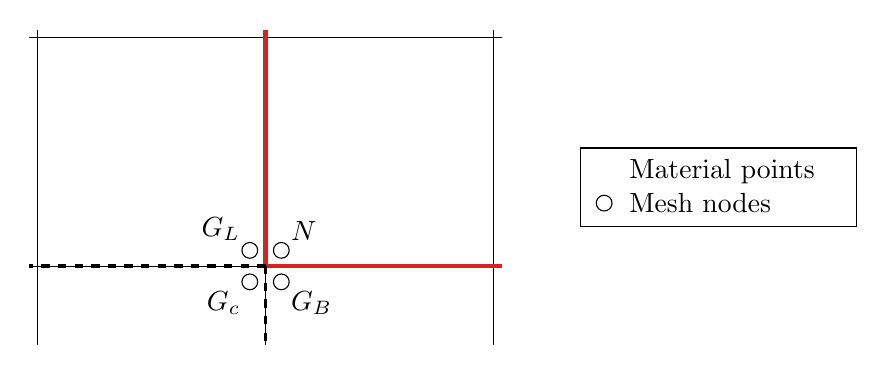
\begin{tikzpicture}
  \draw[step=2.9,black,thin] (-3.,-1.) grid (3,3.);
  \draw[ultra thick,Red] (0,3.) -- (0,0) -- (3.,0);
  % \draw[very thick,white] (0,0)--(0,-1.);
  % \draw[very thick,white] (0,0)--(-3.,-0.);
  \draw[very thick,dashed] (0,0)--(0,-1.);
  \draw[very thick,dashed] (0,0)--(-3.,-0.);
  \fill[white] (-0.2,-0.2) circle (0.1) node [below left] {$G_c$};
  \fill[white] (0.2,-0.2) circle (0.1) node [below right] {$G_B$};
  \fill[white] (-0.2,0.2) circle (0.1) node [above left] {$G_L$};
  \fill[white] (0.2,0.2) circle (0.1) node [above right] {$N$};    
  \draw[black] (-0.2,-0.2) circle (0.1) node [below left] {$G_c$};
  \draw[black] (0.2,-0.2) circle (0.1) node [below right] {$G_B$};
  \draw[black] (-0.2,0.2) circle (0.1) node [above left] {$G_L$};
  \draw[black] (0.2,0.2) circle (0.1) node [above right] {$N$};    
  \cross{0.3}{1.5};\cross{1.}{0.75};\cross{2.}{0.5};\cross{1.}{2.};
  \cross{2.5}{1.75};
  \draw (4.0,0.5) rectangle (7.5,1.5);
  \fill[white] (4.3,0.8) circle (0.1) node [right,black] {\: \text{Mesh nodes}};
  \draw[black] (4.3,0.8) circle (0.1);
  \cross{4.3}{1.2};
  \node[right] at (4.3,1.2) {\: \text{Material points}};
\end{tikzpicture}
  \caption{Corner ghost nodes in a two-dimensional DGMPM mesh.}
  \label{fig:corner_ghost}
\end{figure}
Transverse corrections further require the introduction of corner ghost nodes equivalent to finite volume corner cells \cite{Leveque}. Consider the two-dimensional case depicted in figure \ref{fig:corner_ghost} in which boundary edges are represented by red lines.
%First, boundary interfaces are extended to the corner cell (vertical and horizontal dashed lines).
First, an inverse Riemann problem is solved between the corner ghost node $G_c$ and one regular ghost node, say $G_B$, so that the stationary solution of the Riemann problem between those ghost nodes corresponds to the boundary condition holding on the vertical edge.
Second, this procedure is repeated between the corner ghost node and $G_L$ in order to enforce the boundary condition holding on the bottom boundary between them.

\begin{remark}
  \label{rq:BC_ghostnode}
  The solution of Riemann problems involving ghost nodes is made possible by extending material properties of the adjacent cell so that the characteristic structure of the solution can be computed. This implies that the deformation of interior nodes is duplicated to ghost nodes for problems such as hyperelasticity, which eigenstructure depends on the deformation gradient. Hence, for such problems ghost nodes may carry stress and strain that are not related by constitutive equations. However, the deformation gradient at ghost nodes has no physical sense and is only used to compute the correct wave speeds.
\end{remark}

\subsection{DGMPM solution scheme}
Let us assume that the vector of specific conserved quantities $\bar{\Ucb}^n$ as well as the auxiliary vector $\Qcb^n$ are known at every material points that discretize a continuum body $\Omega_0$, in a grid made of $N_{n}$ nodes at a given time $t^n$. The computational procedure followed within the DGMPM between two time steps $n$ and $n+1$ can now be derived. We consider here cases based on the use of an auxiliary vector, the others being only particular cases.
% , which requires to (i) solve the hyperbolic system \eqref{} in $\Omega$ with associated boundary conditions and (ii) update the vector $\bar{\Qcb}^n$ on material points.

The scheme has been established with a total Lagrangian formulation, therefore, the lumped mass and \textit{pseudo-stiffness} matrices $M^L_{ij}$ and $K^\alpha_{ij}$ of the semi-discrete form \eqref{eq:DGMPM_semi_discrete} are computed once and for all at the beginning of the calculation. The procedure then reads:
\begin{itemize}
%\item[] $\bar{\Ucb}, \:\Qcb$ known at material points
\item[(a)] The discrete equation \eqref{eq:DGMPM_discrete} and Riemann problems at cells interfaces \eqref{eq:RP_quasilinear} require a projection of fields onto the grid:
  \begin{equation}
    \label{eq:DGMPM_points2nodes}
    M^L_i \bar{\Ucb}^i = \sum_{p=1}^{N_p} S_{ip} m_p \bar{\Ucb}^p \qquad \text{and} \qquad M^L_i \vect{\Qc}^i = \sum_{p=1}^{N_p} S_{ip} m_p \vect{\Qc}^p 
  \end{equation}
  to be solved for each $\bar{\Ucb}^i$ and $\vect{\Qc}^i$ respectively. The projection of fields from particles to nodes hence follows the weighted least squares interpolation used in MPM. 
%\item[(b)] Compute time step: in the general case the tangent modulus depends on the deformation gradient as well as the waves speeds. It is therefore needed to compute the time step so that the fastest wave can at most cross the smallest cell of the mesh according to Courant condition.
\item[(b)] The specific flux vectors $\bar{\Fcb}^i_{\alpha}$ involved in the equations are computed from $\vect{\Qc}^i$ knowing $\rho_0$, thus avoiding the computation of constitutive equations.
\item[(c)] Enforcement of boundary conditions on ghost nodes.
\item[(d)] Computation of interface fluxes: 
  \begin{itemize}
  \item[1-] Build the state vectors $\vect{\Qc}_{X_N^{\pm}}$ based on $\vect{\Qc}^{i,n}$ where $i$ denotes the nodes belonging to the face on both sides of an interface.
  \item[2-] Compute the stationary solution $\Qcb^*$ by means of the approximate-state Riemann solver.
  \item[3-] Calculate the corresponding Godunov flux $\Fcb_N \(\Qcb^*\)$ by either using the DCU or the CTU approach.
  \end{itemize} 
\item[(e)] Advance solution in time by solving the discrete equation \eqref{eq:DGMPM_discrete} at each node.
\item[(f)] Back-mapping: as motivated at the end of section \ref{sec:MPM}, the nodal updated solution is projected to material points with the classical interpolation as in PIC:
  \begin{equation}
    \bar{\Ucb}^{p,n+1} = \sum_{i=1}^{N} S_{ip}\bar{\Ucb}^{i,n+1}
  \end{equation}
\item[(g)] Material point kinematics and constitutive model: The new solution $\bar{\Ucb}^{p,n+1}$ allows to increment the deformation $\vect{\varphi}(\vect{X},t)$ and to update stress components, which will be used in the auxiliary vector for the next time step, through hyperelastic constitutive equations:
  \begin{align}
    & \vect{\varphi}^{p,n+1} = \vect{X}^p + \Delta t \vect{v}^{p,n+1} \\
    & \tens{\Pi}^{p,n+1} =  \drond{\Psi}{\tens{F}}(\tens{F}^{p,n+1})
  \end{align}
  The grid may then be discarded and reconstructed and in particular by means of adaptive algorithms applied in the reference configuration, in order to improve wave front tracking in the current one.
\end{itemize}

Let's now recall or highlight significant differences between the DGMPM and the original MPM schemes. 
% Ouai ?
%First, while the DGMPM uses a classical interpolation to mapping back the updated solution to material points (step f), FLIP method and MPM require an additional time integration on material points. 
% ok
First, the use of conservation laws \eqref{eq:conservative_form} instead of the momentum equation in the weak form implies that both velocity and gradients are solved at nodes making this new approach close to finite volume methods, which provides the same order of accuracy for both fields. 
% ok
Next, since the deformation gradient is no longer calculated with shape functions gradients, the task of choosing between USF and USL algorithms vanishes. In that sense the DGMPM scheme is simpler.
At last, the solution of Riemann problems at every edges of the mesh increases computational time. Fortunately, the use of discontinuous Galerkin approximation makes this numerical method highly parallelizable \cite{Cockburn}.

The numerical scheme derived above is analyzed in terms of stability and convergence in the next section.


%%% Local Variables: 
%%% mode: latex
%%% TeX-master: "../mainManuscript"
%%% End:
